\documentclass[a4paper,11pt]{article} % options in brackets are not required; 10pt is standard in article
\usepackage{amsmath} % package offers specialized environments for writing multi-line formulas
\usepackage{graphicx}
\begin{document}
\title{%
  \large Seminar Development \& Growth \\
  \huge Modelling assignment: Education Policy}
\author{Anne van de Vorst and Bart de Geus}
\date{March 17, 2016}
\maketitle


\section{Introduction}
In this modeling assignment we will introduce a subsidy to education in the model used in section 13.3.2 of Aghion and Howitt (2009). In section 13.3.2 Aghion and Howitt describe a model that was inspired by Acemoglu (1997) and Redding (1996). The model looks at the composition of education spending and the way it interacts with the level of technological development in a country. Individuals make a decision regarding the amount of investment in education in period 1. At the same time, entrepreneurs decide how much they would like to invest in innovation. These decisions depend on the expected level of productivity growth and the expected level of human capital respectively. Thus, the decisions depend on the decision of the other party and as a result of this interaction; there are multiple growth paths; a low-growth equilibrium and a high-growth equilibrium. Since it is hard to leave the low growth equilibrium this equilibrium is often called a low-development trap. Here, we will introduce subsidies on education and see what the result of this subsidy is on the equilibriums and whether this might be a solution for the low-development trap. First, we will give an overview of the model in section 13.3.2.

\section{Overview model 13.3.2}
\subsection*{\textit{Individuals}} % * cancels numbering of section or subsection
In this model all individuals live for two periods and are born with a level of human capital that is equal to one. Individuals, as in most models, maximize their utility, with a discount factor for consumption in the future since they value consumption today more than consumption tomorrow.
 
\begin{equation}
  \underset{\nu}{max}\{u\}=\underset{\nu}{max}\{c_1+\rho c_2\}
\end{equation}

The consumption functions of the individuals are the earnings of the young in every period. These function are given by the following formulas:

\begin{equation}
  c_{young,t}=(1-\nu_t)A_t
\end{equation}
\begin{equation}
  c_{old,t+1}=\beta A_{t+1}h_{old,t+1}
\end{equation}

The earnings of individuals when they are young equal the amount of production time times the existing leading-edge technology, since this is the amount they produce when they are self-employed. Human capital is present in equation (2) but it is normalized to one. Here we assume that individuals work for a firm when they are old. Old individuals earn a fraction of the output surplus in which the level of human capital and the level of the leading-edge technology determine this output surplus. Individuals cannot decide upon the level of the leading-edge technology but they can influence their level of human capital when they are old. When they invest in education when they are young, their human capital when they are old will be higher than the level of human capital when they were young. The more they will invest in education, the higher the increase in human capital is; this is formulated in equation (4).

\begin{equation*}
  h_{2,t}=1+\gamma\nu^{\theta}
\end{equation*}
\begin{equation}
  h_{2,t}=1+\gamma\left(\left[\beta\rho\theta\gamma\left(\mu\lambda+1-\mu\right)\right]^{\frac{1}{1-\theta}}\right)^{\theta}
\end{equation}

Thus, there is a trade-off between the costs (decrease in production time when young) and the benefits (increase in human capital when old) of education. When individuals maximize their utility, they make a decision regarding the fraction of their working time they want to invest in education when they are young. 
After inserting the equation for human capital (4) in the consumption function (3) and inserting the consumption functions (2) and (3) in the utility function (1) it is possible to maximize the utility function with respect to \(\nu\). Rewriting this first order condition gives:

\begin{equation}
  \nu^{*}=\left[
    \frac{1}{\rho\beta
      \left[\mu\lambda+1-\mu\right]
    \theta\gamma}
  \right]^{\frac{1}{1-\theta}}
\end{equation}

Equation (4) shows the optimal fraction of working time individuals invest in education. When individuals invest this fraction in education their utility is maximized. As equation (4) shows this fraction depends on the \textit{expected} productivity growth in the country. When individuals expect that the productivity growth will be high, they will invest more in education. Figure 1 shows this correlation between expected productivity growth and the level of human capital.

\begin{figure}
  \centering
  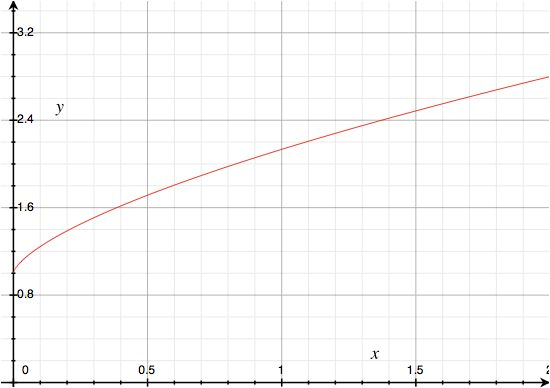
\includegraphics{figure1.png}
  \caption{Level of human capital on expected productivity growth}
\end{figure}

\subsection*{\textit{Entrepreneurs}}
Entrepreneurs face a decision regarding the amount they want to invest in innovation. Investing in innovation costs money but it will increase the output surplus. Entrepreneurs maximize their profit that is given by the following formula:

\begin{equation}
\underset{\mu}{max}V(\mu)=
\underset{\mu}{max}
  \left\{-\mu\alpha A+\rho\left(1-\beta\right)\left(\mu\lambda+1-\mu\right)\left(1+\gamma\nu^{\theta}\right)A\right\}
\end{equation}



\end{document}
